\subsection{PIMS Artificial Intelligence Module}
This module is responsible for predicting the chances of survival for each cancer type. Parameters for each patient are considered to compute this prediction. These parameters are converted into a single value that will be used by the PIMS Neural Network Module as input. \par 

\subsubsection{Scope}
The scope is shown in the use case diagram below: \par
\begin{figure}[H]
\centerline{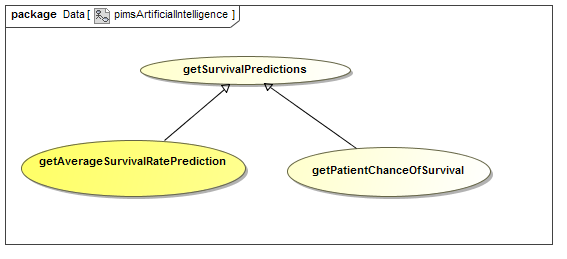
\includegraphics[width=0.75\linewidth]{./Functional_Requirements/Graphics/pimsAI/pimsArtificialIntelligence}}
\caption{The global scope for PIMS Artificial Intelligence Module}
\end{figure}

\subsubsection{Use cases}
\begin{description}

	\item{\textbf{getAverageSurvivalRatePrediction -- [priority: critical]}}
	\begin{description}
		\item{\textbf{Service Contract}} The generic service contract
		\begin{figure}[H]
			\centerline{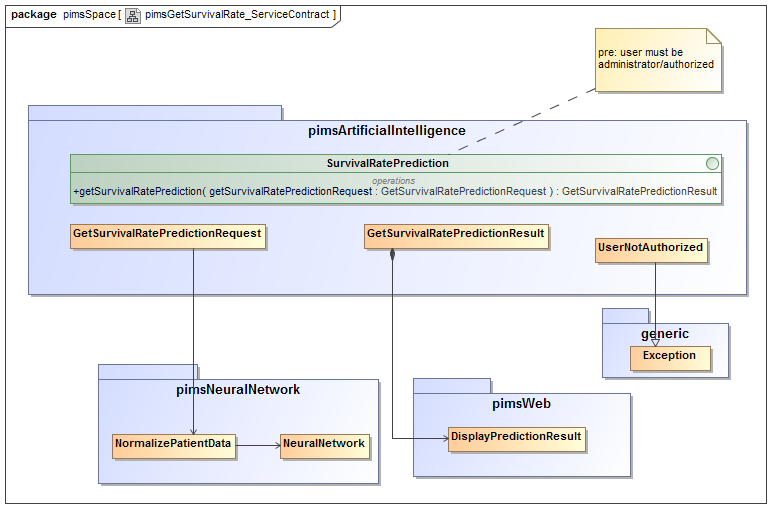
\includegraphics[width=0.8\linewidth]{./Functional_Requirements/Graphics/pimsAI/pimsGetSurvivalRate_ServiceContract}}
			\caption{Service contract for getAverageSurvivalRatePrediction}
		\end{figure}
	\end{description}
	
		\item{\textbf{getPatientChanceOfSurvival -- [priority: critical]}}
	\begin{description}
		\item{\textbf{Service Contract}} The generic service contract
		\begin{figure}[H]
			\centerline{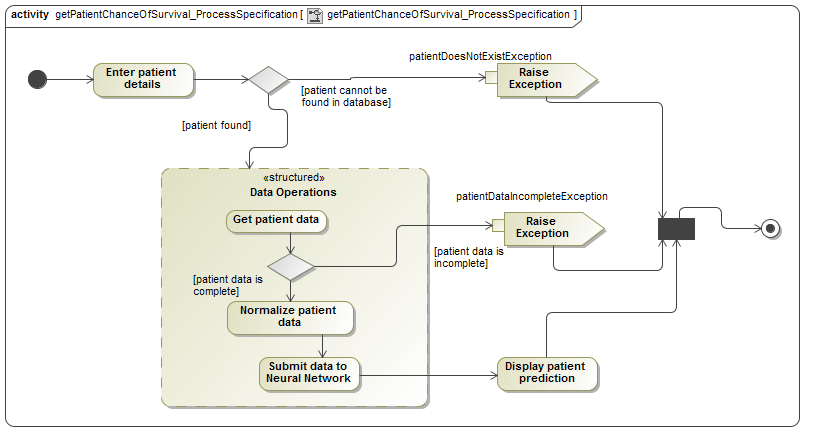
\includegraphics[width=0.9\linewidth]{./Functional_Requirements/Graphics/pimsAI/getPatientChanceOfSurvival_ProcessSpecification}}
			\caption{Process specification for Service contract for getPatientChanceOfSurvival}
		\end{figure}
	\end{description}
\end{description}

	\subsubsection{Neural Network Training}
	Patient data was analysed for possible risk factors for cancer susceptibility. These risk factors are:
	\begin{itemize} %Lindelo you can add the paramters used and explain how you normalized each one with justifications
		\item Age - No normalization was required for this field. However, decimal scaling was used for the age. Patients are expected to be within the age range of [16 - 100] so the age is scaled-down to two decimal places.
		\item HIV status - Is a binary field (either negative or positive). Negative HIV statuses were given the numerical equivalent of 0.9 while a positive status holds 0.1.
		\item CD4 count (If HIV status is positive) - If the patient is HIV negative, the numerical values becomes 0.9998. Otherwise, decimal scaling (4 places down) is used since the CD4 range is 0 - 1500.  
		\item Figo Stage - Since this value is neither binary nor numeric, the number of figo stages determines how the patient's stage is normalized. If there are n stages then the kth stage gets the numerical equivalent of : \(\frac{k-stage}{n}\)
		\item Site of distant metastase - Same as the Figo stage. 
		\item Histology - Also uses the same concept as Figo stage.
		\item Differentiation - Also uses the same concept as Figo stage.
		\item Primary treatment -  Also uses the same concept as Figo stage.
		\item Type of surgery - Also uses the same concept as Figo stage.
		\item Type of radiotherapy - Also uses the same concept as Figo stage.
		\item Response to treatment - Also uses the same concept as Figo stage.
		\item Relapse - Also uses the same concept as Figo stage.
		\item Last known vital status - Also uses the same concept as Figo stage.
		
	\end{itemize}
	
	The Neural Network makes use of the back-propagation algorithm for the purpose of learning.

	\begin{itemize}
		\item The equations used for the neural network are as follows:
		\begin{itemize}
			\item Input Function:
			 \[net =\sum_{i=1}^{n} {x_i} {w_i}\]
			 
			 \item Hidden layer Input Function:
			  \[net_{y_i} =\sum_{i=1}^{I + 1} {z_i}{w_ji}\]
			  
			  \item Hidden layer Sigmoid Activation function:
			  
			  \[y_j =\frac{1}{1 + {e}^{-net_{y_j}}}\]
			  
			   \item Output layer Input Function:
			  
			  \[net_{o_k} =\sum_{j=1}^{I + 1} {y_j}{w_kj}\]
			  
			  \item Output layer Sigmoid Activation function:
			  
			  \[o_k =\frac{1}{1 + {e}^{-net_{o_k}}}\]			  
			
			\item Sigmoid Activation function: \[f(net) =\frac{1}{1 + {e}^{-net}}\]
			
			\item Training error: \[Error =(t_k - o_k)\]
			
			

		\end{itemize}
		
		\begin{itemize}
		\item The equations used for the back propagation phase are as follows:
			\begin{itemize}
				\item Output layer error propagation:
				 \[\delta_{o_k} = -(t_k - O_k)(1 - O_k)O_k\]
				 
				 \item Output layer weights propagation:
				 \[w_{k_j}{o_k} \mathrel{+}= -(\delta_{o_k}y_j\]

				 \item Hidden layer error propagation:
				 \[\delta_{y_j} = -(w_{k_j} \delta_{o_k} (1-y_j)y_j\]				 
				 
				 \item Hidden layer weights propagation:
				 \[v_{j_i} \mathrel{+}= \delta_{y_j}z_i\]
				 

			\end{itemize}
		\end{itemize}
	
	\end{itemize}
	
	
	\subsubsection{Neural Network Testing}
	When testing the network, a the critical cancer parameters are normalized given a patient name. When classifying the patient as likely to survive or die form cancer the principles of a statistical probability density function, ${\rchi^2}$-distribution are applied; wherein the null hypothesis is \setlength{\thinmuskip}{0mu} (\textbf{$H_0$}):
	\begin{itemize}
		\item A patient is likely to survive cancer
	\end{itemize}
	 in order to obtain a confidence interval for the survival prognosis. A 50\% significance level is used for the confidence interval; such that 50\% of the time, the output node value is likely to be a false positive and as for the other percentage, one can be confident in it as being accurate. The choice of the application of the ${\rchi^2}$-distribution is plainly for it's simplicity and it is a well known probability density function. The choice of the confidence interval was aided by the application of artificial neural networks in survival analysis when compared with other survival analysis statistical models \cite{BeyondtheCoxmodel}.
	
	\begin{itemize}
		\item The below ${\rchi^2}$-distribution formulas are used:
		
		\begin{itemize}
			\item Probability: \footnote{\textit{n} is the number of patients to test, \textit{E} is the target, \textit{O} is the output node value, \textit{k is the individual patient}}
			\[\chi^2=\frac{1}{d}\sum_{k=1}^{n} \frac{(O_k - E_k)^2}{E_k}\]
			\item Confidence interval: \footnote{\textit{s} is the mean square error}
			\[\pm    \frac{(n-1) \times s^2}{\chi^2_{\frac{\alpha}{2}} \times (n-1)}\]
			\item Degrees of freedom: \[(n-1)\]
		\end{itemize}
		\item The ${\rchi^2}$-distribution table of critical values will be used to test (\textbf{$H_0$})		
			\begin{figure}[H]
			\centerline{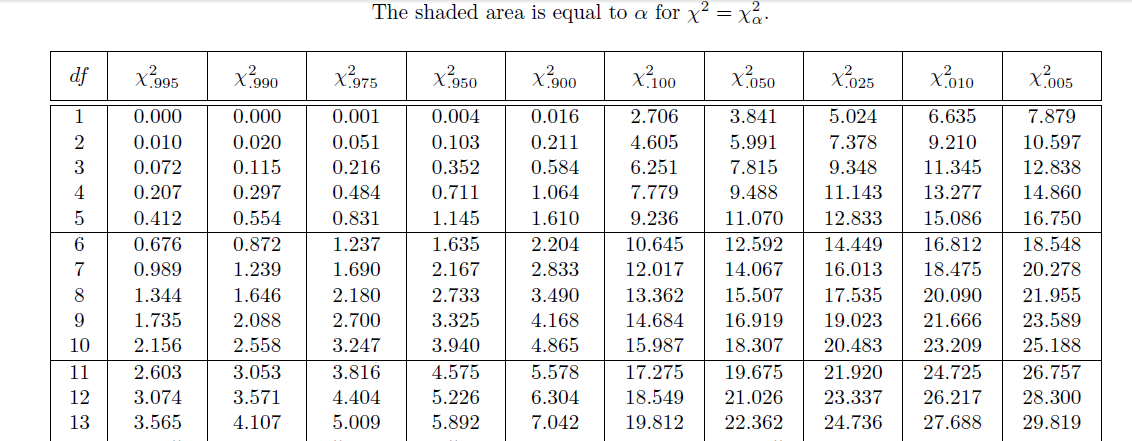
\includegraphics[width=0.8\linewidth]{./Functional_Requirements/Graphics/pimsAI/Chi_image}}
			\caption{Snippet of Chi-squared distribution critical value table}
		\end{figure}
		
		
	\end{itemize}

